\section{CEBAF Accelerator}

The Continuous Electron Beam Accelerator Facility (CEBAF) accelerator is a recirculating accelerator at Thomas Jefferson National Accelerator Facility (JLab). That is, there are two linear accelerators (linacs) connected by recirculation arcs. CEBAF has recently undergone an upgrade which increased the maximum possible energy to 12 GeV (to Hall D). The 12-GeV configuration of CEBAF can be seen in Figure \ref{fig:cebaf}. Electrons traveling through both linacs a single time is called a ``pass''. Halls A, B, and C are capable of receiving up to 5-pass beam; Hall D can receive up to 5.5-pass beam. The beam provided is Continuous Wave (CW), comprised of a steady stream of electrons, rather than many electrons in short pulses.

\begin{figure}[h]
\begin{center}
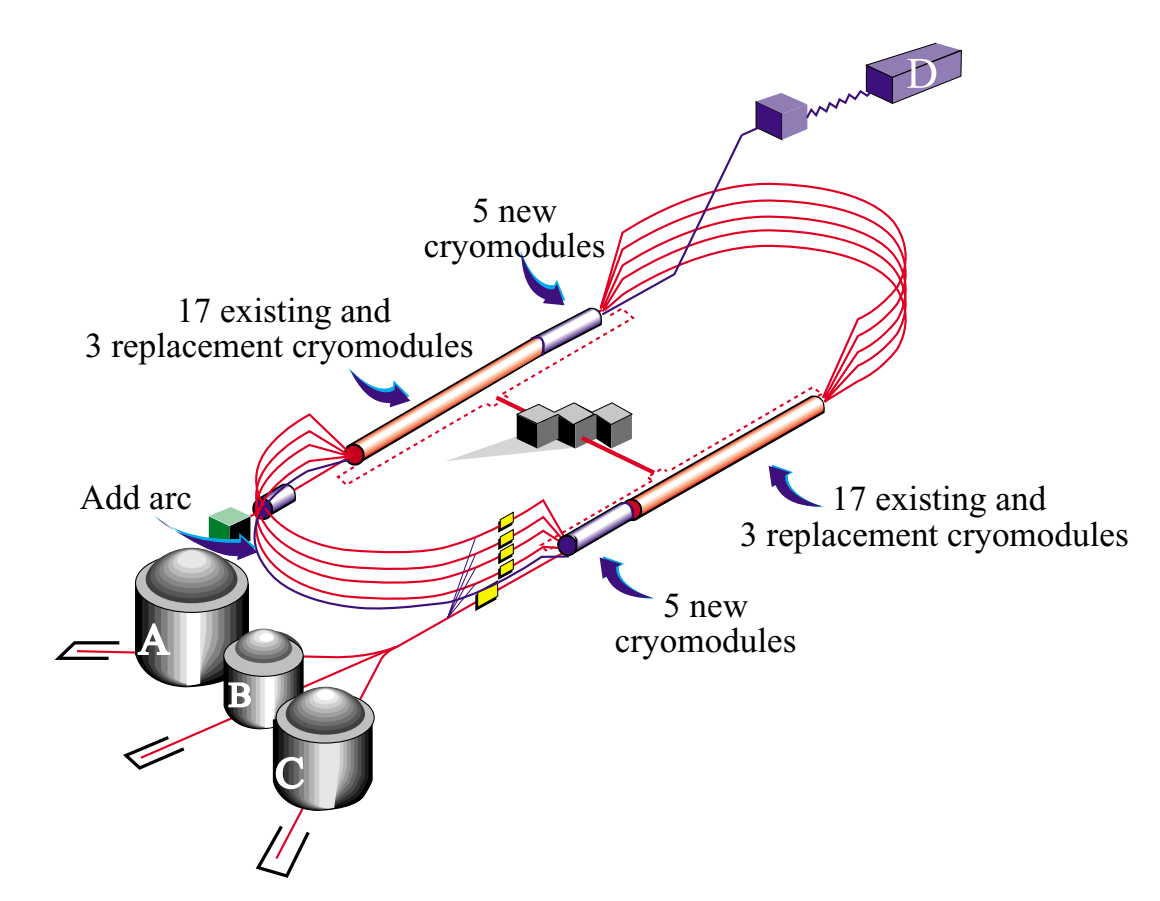
\includegraphics[width=0.7\textwidth]{./setup/fig/cebaf.png}
\caption{The current 12-GeV configuration of the CEBAF accelerator with the upgrades that were made from the 6-GeV configuration \cite{12gevWP}.}
\label{fig:cebaf}
\end{center}
\end{figure}
